    \subsection*{Weaknesses of $k$-means}
    
        There are some \textbf{weaknesses} to $k$-means clustering. Certain patterns that we can \textbf{see} aren't easily \textbf{clustered}.
        
        We can see this with a few \textbf{examples}:
        
        \begin{figure}[h]
            \centering
            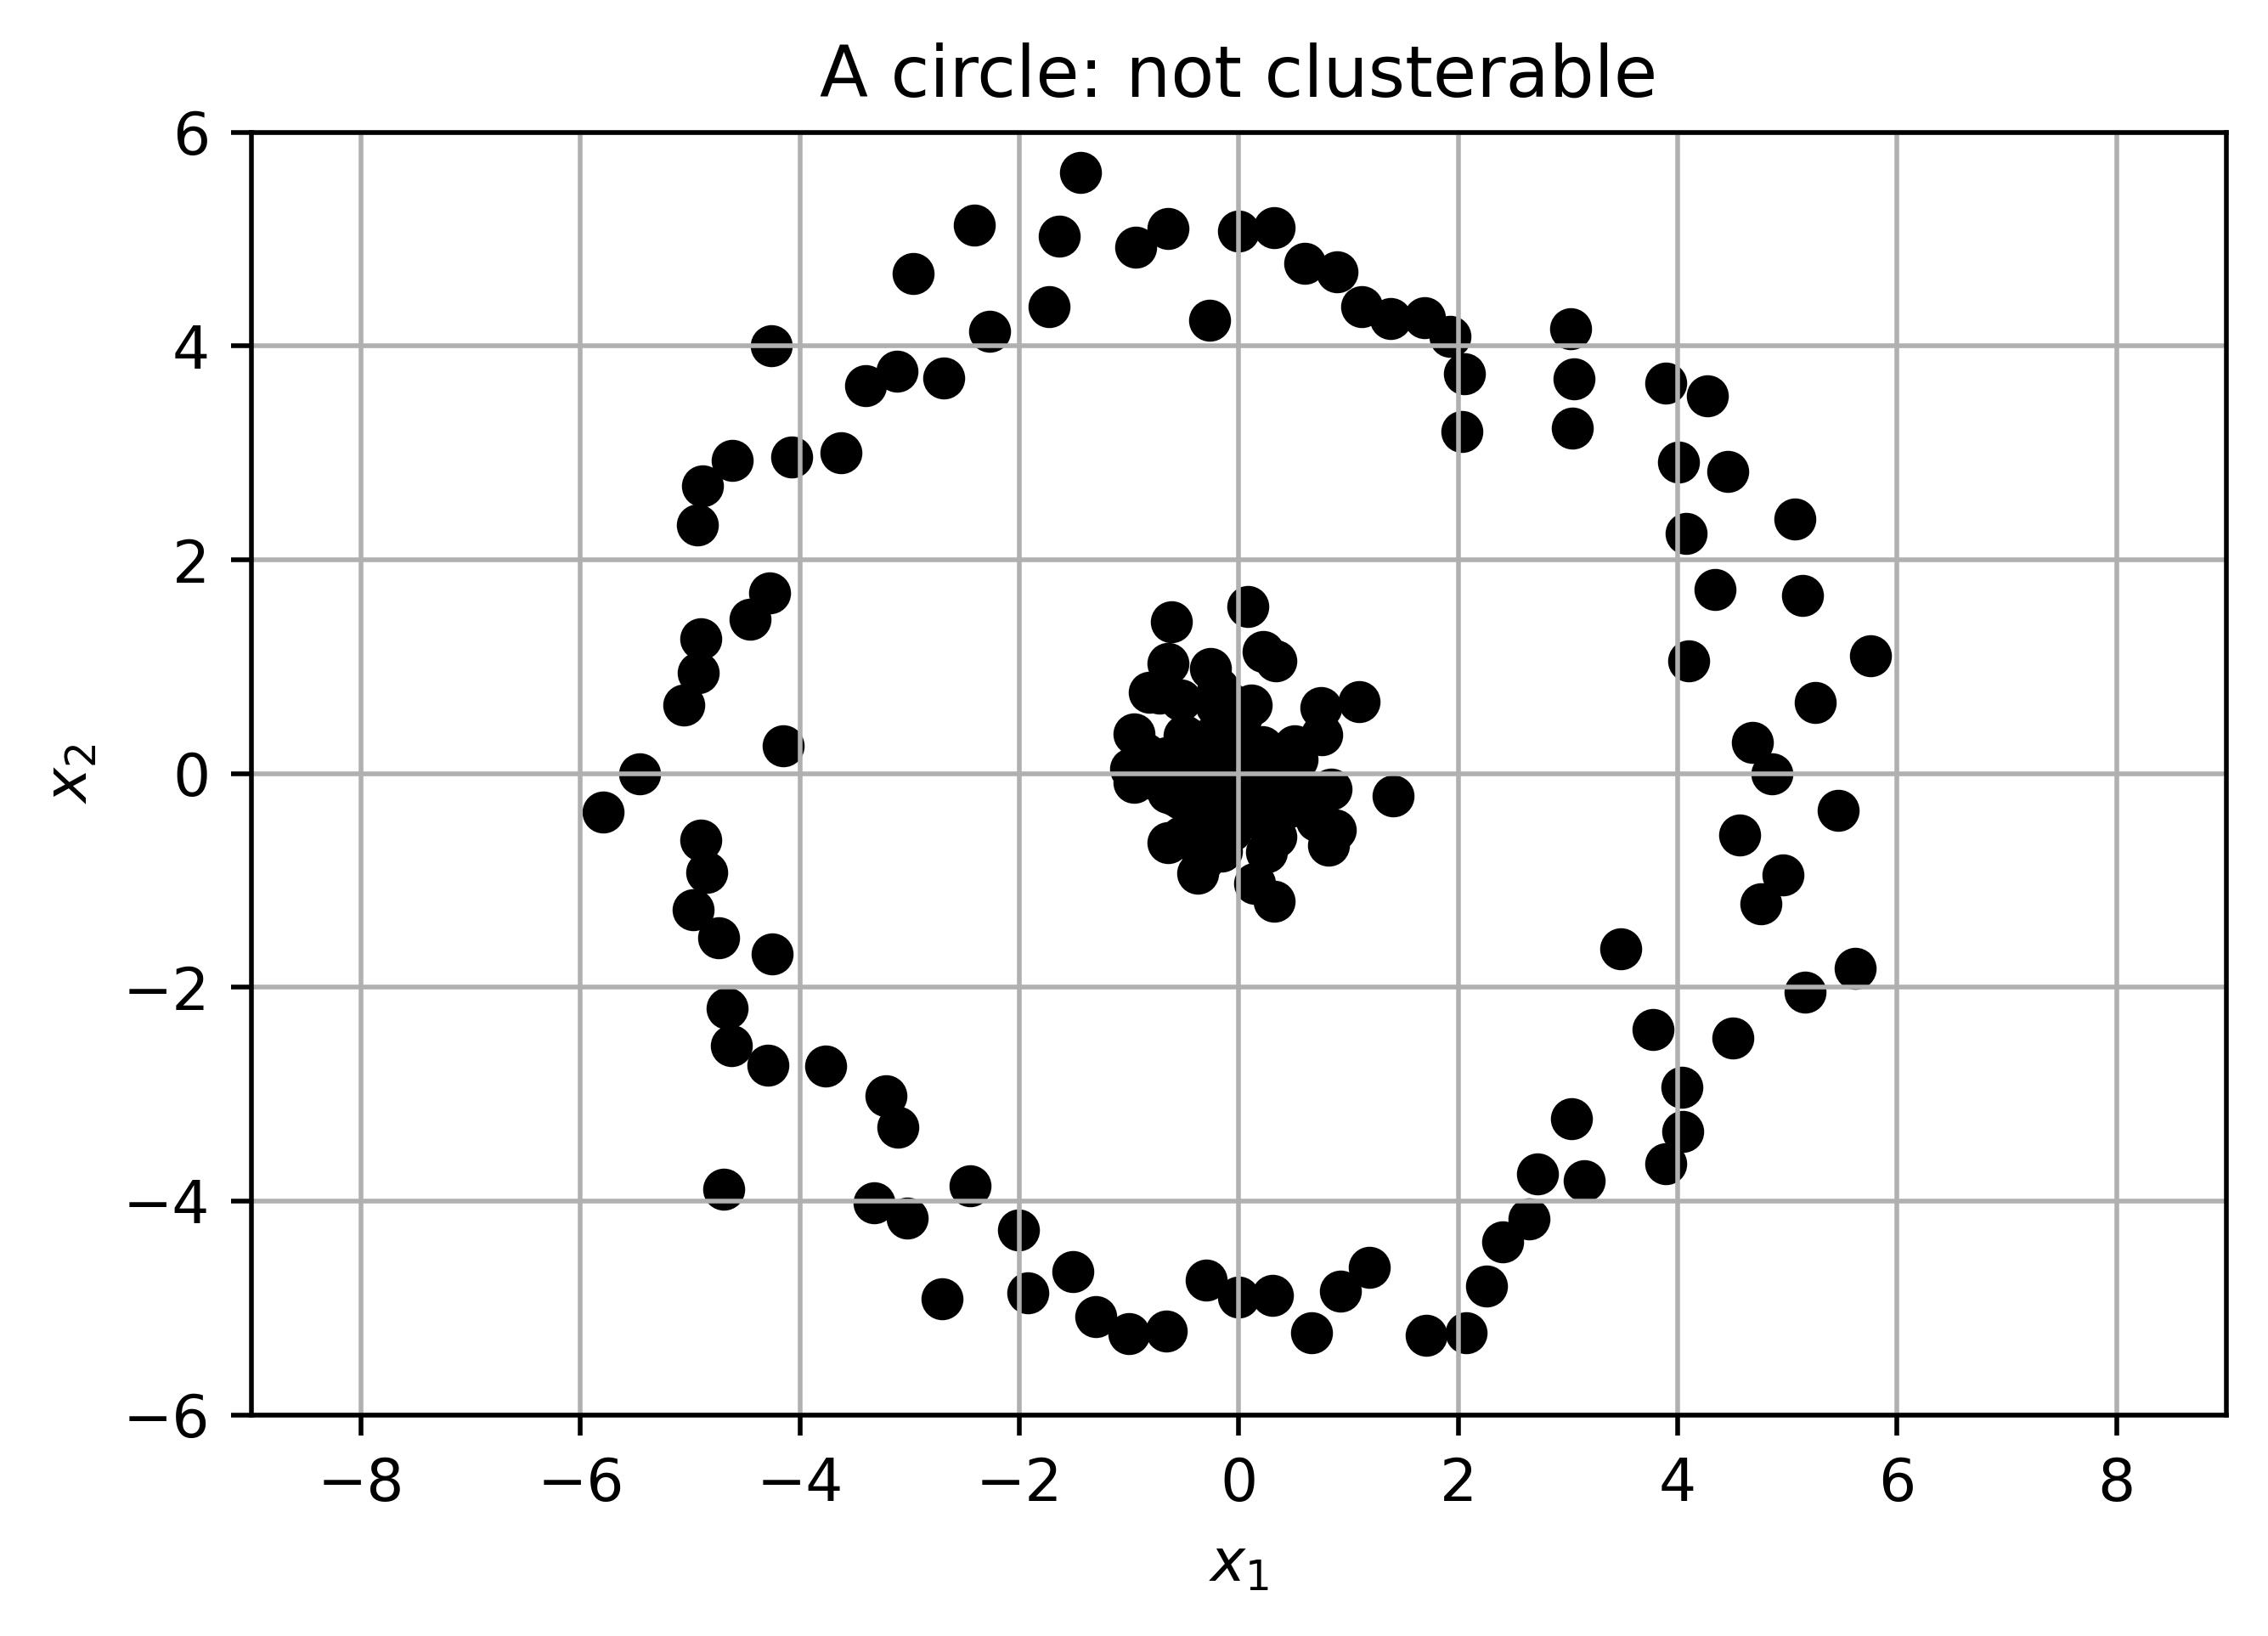
\includegraphics[width=0.65\textwidth]{images/clustering_images/center_unclusterable.png}
            \caption*{This data can't be simply clustered.}
        \end{figure}
        
        This example can't be effectively \textbf{clustered}: most people would agree that the "outer ring" should be \textbf{one} cluster, while the "inner circle" should be \textbf{another}.
        
        But, assuming we (correctly) place one cluster mean in the \textbf{center}, there's \textbf{nowhere} we can put our other cluster mean to be \textbf{closest} to all of the \textbf{outer} points, but \textbf{not} the inner points.
        
        We might be able to \textbf{resolve} this using a \textbf{feature} transformation. But, the problem remains.
            \note{For example, we could have a feature represent the radius! But then, we would still struggle with a ring not centered on the origin.}
            
        Another example works for clusters that aren't very centralized:
        
        \begin{figure}[h]
            \centering
            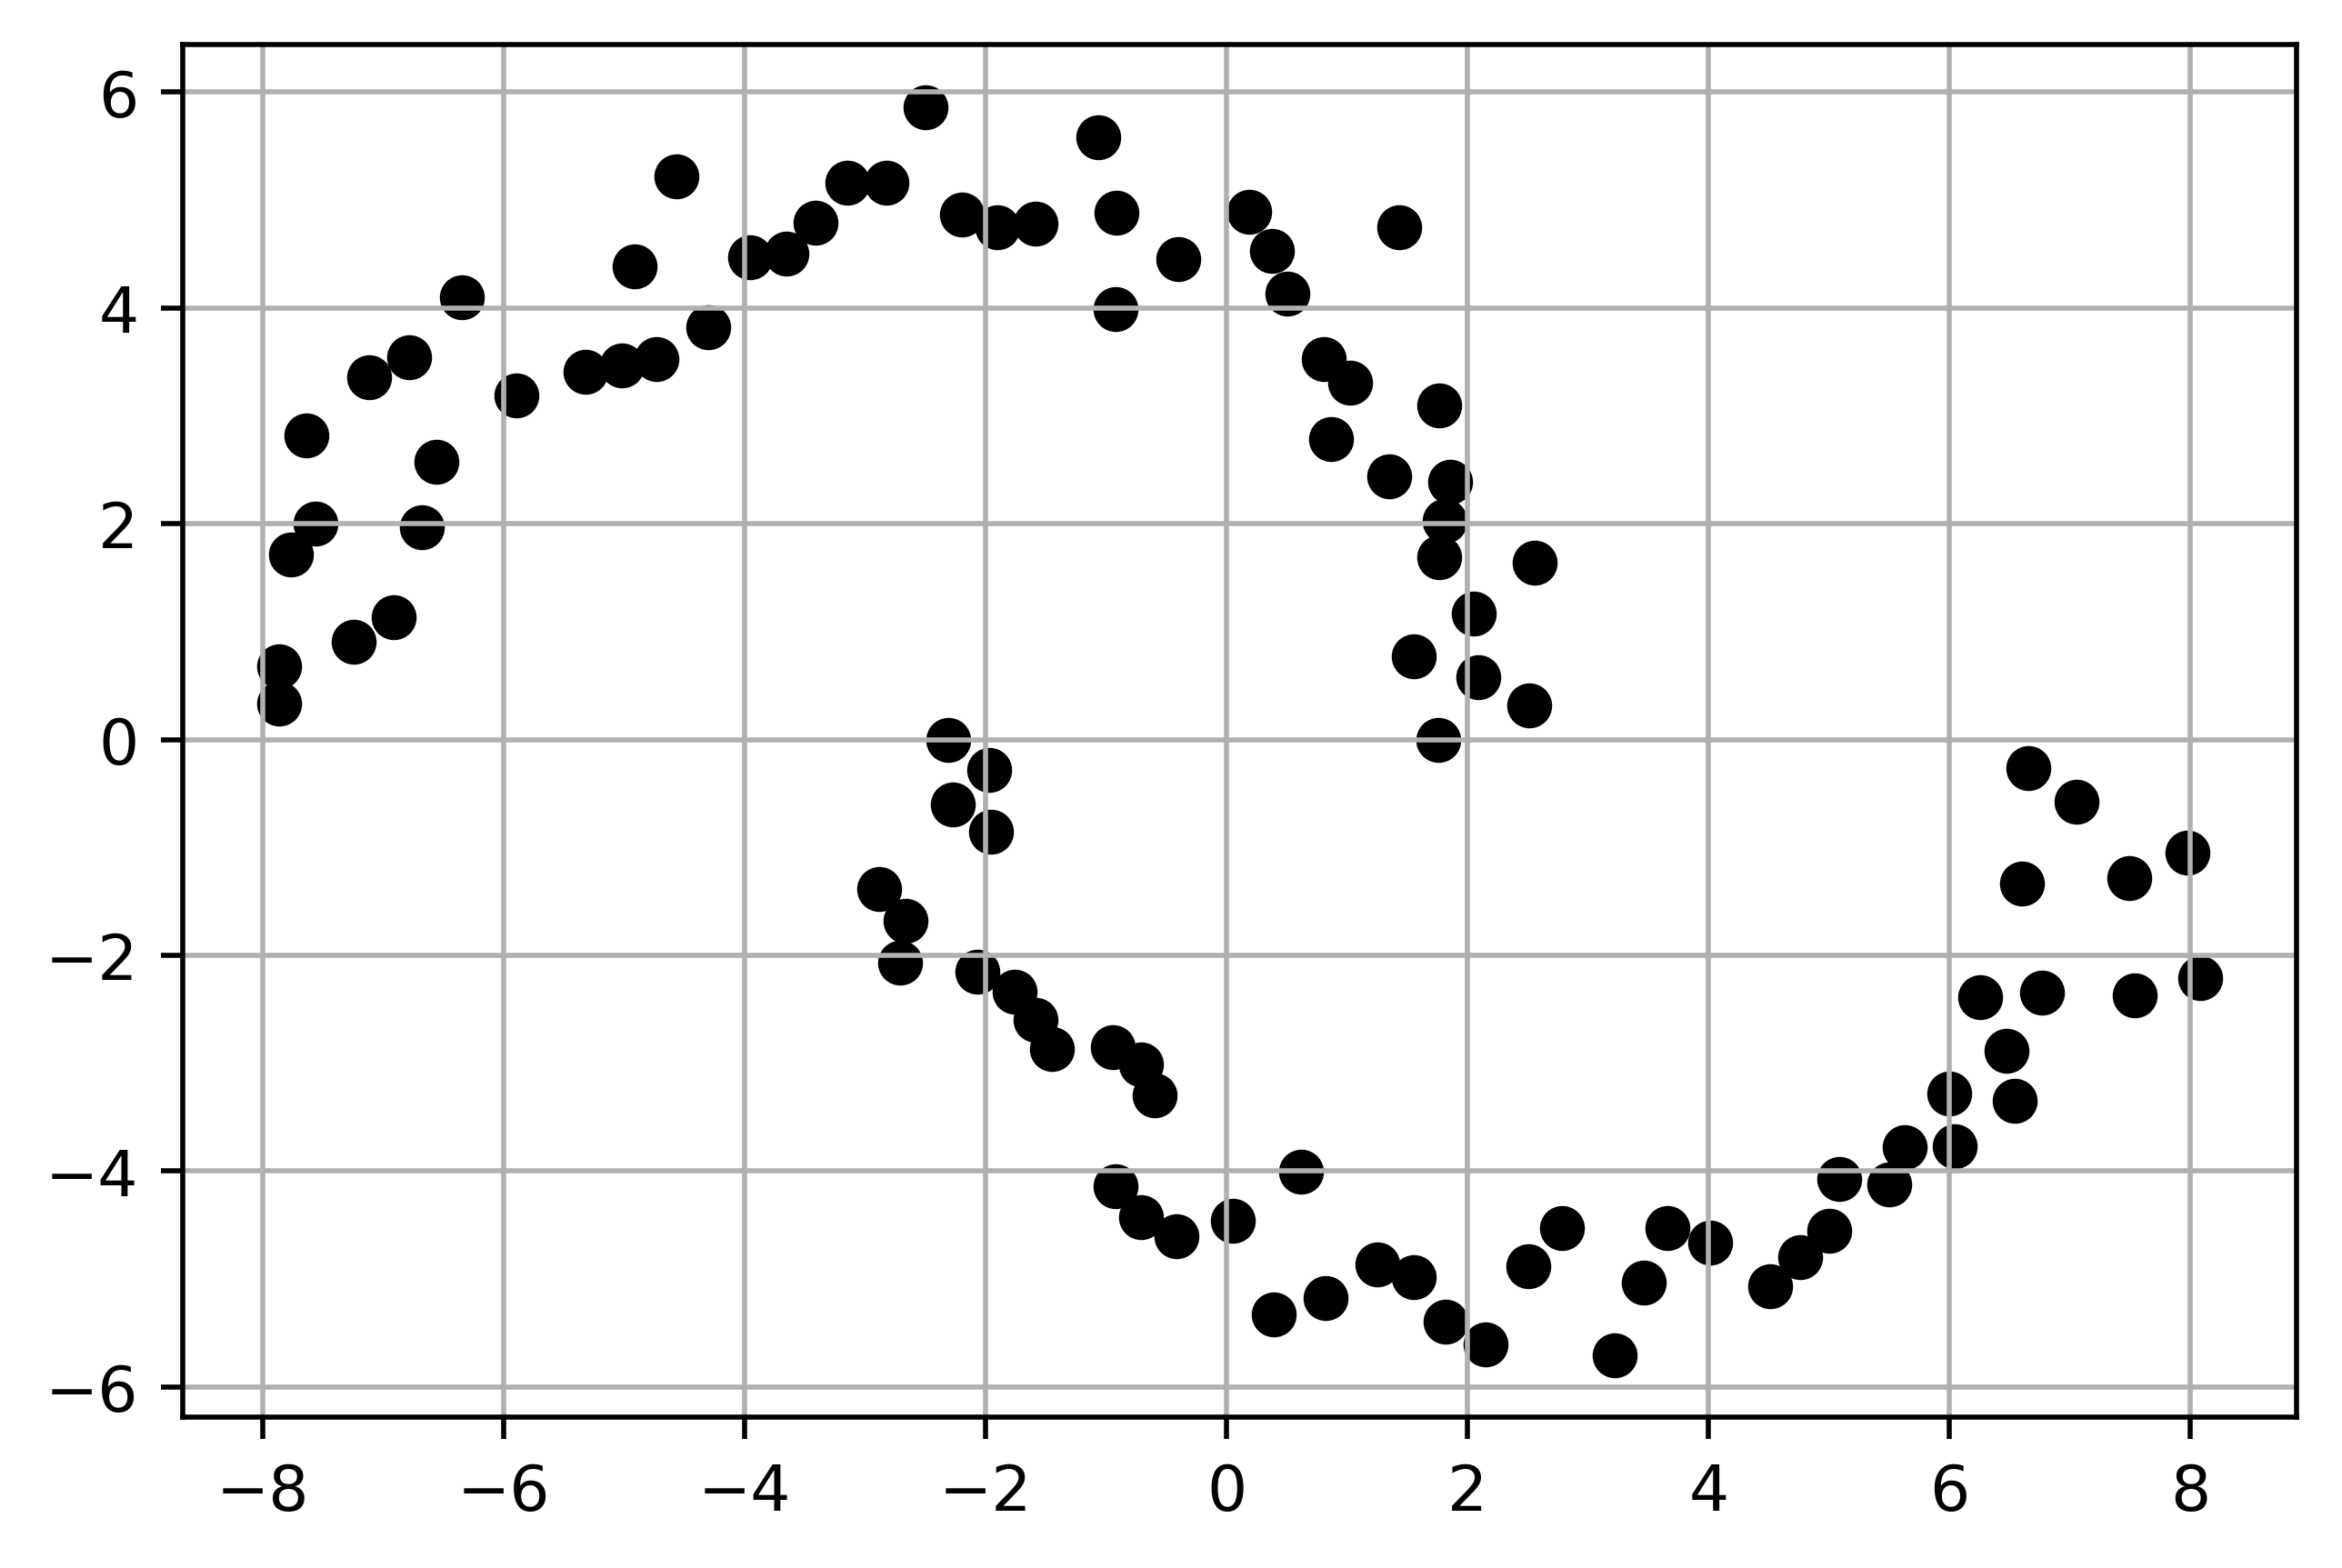
\includegraphics[width=0.65\textwidth]{images/clustering_images/offset_unclusterable.png}
            \caption*{This data can't be clustered either!}
        \end{figure}
        
        The edge of one cluster is too close to the other: we can't easily create a good pair of cluster means for each semi-circle.